



In this section, we evaluate the different GPU-based scheduling schemes for four major criteria: (i) Cluster-wide utilization, (ii) QoS violations, (iii) Power, and (iv) Accuracy of prediction.


\subsection{Cluster-wide GPU Utilization}
Building upon the uniform scheduler which does GPU-agnostic scheduling (shown in Figure~\ref{fig:uniform}), we propose three scheduling schemes: (i) Res-Ag (ii) CBP and (iii) PP. In Figure~\ref{fig:pcp}, we plot the  utilization improvements of each of the ten GPU nodes for every app-mix using the PP scheduler. The PP scheduler improves the utilization in all the three app-mixes by an average of 62\%. Especially in app-mix 2 and app-mix 3, where the utilization is medium and low respectively, the PP scheme does an effective consolidation of workloads using a minimal number of GPUs as possible. As seen in Figure~\ref{fig:app3-pcp}, GPU nodes 1,4,8 and 10 are minimally used as the scheduler effectively consolidated all the low demand workloads to a minimum number of active GPUs as possible. This consolidation shows that, PP leverages the real-time utilization along with utilization forecasting before making any scheduling decisions. 

Figure~\ref{fig:util} plots the overall resource utilization improvements for all three application mixes for median and tail percentiles. It can be noted that our PP scheme consistently improved the overall GPU utilization in all low, medium and high application-mix cases. For example, PP in app-mix-1 improves by 80\% for both median and tail percentiles when compared with Res-Ag scheduler. The improvements are also consistent in the other two app mixes where the improvement over Res-Ag scheduler for median and peak percentiles are 60\% and  45\% respectively. These benefits reaffirm our prior observation that, it is better to predict the peak resource consumption of the workloads.

~\subsection{QoS of latency critical workloads}
~\label{sec:qos}
QoS violation threshold for latency-sensitive applications is typically set around 150 milliseconds \cite{Dean}. When end-to-end latency of such queries exceeds 150ms, they have to be relaunched. We show in Figure~\ref{fig:qos} that the baseline scheduler violated QoS by 18\% on average even though the applications are not co-located together. This is because of queuing delays, where the query is sent to a busy GPU node. The Res-Ag performs worse than the baseline and violates the threshold from 10\% (app-mix-3) to 53\% (app-mix-1) of the requests. On the contrary, CBP and PP have almost no violations in all three app-mix ($<$1\%). This is because these schemes were aware of real-time GPU utilization and provisioned the containers for 90 percentile utilization while guaranteeing the QoS via utilization forecasting. 
{Note that, we also co-locate the latency sensitive queries along with the batch jobs without affecting their QoS. PP achieves this by predicting the inter and intra-application correlation for utilization and, at the same time by leveraging Knots real-time data, it can forecast the future node utilization. This avoids QoS violations while keeping the utilization high.}

Since \textit{Knots} exposes the GPU utilization through Nvidia's resource monitoring APIs, the schedulers built on top of \textit{Kube-Knots} inherently take advantage of these metrics. Figure~\ref{fig:load} plots the pair-wise COV of GPU cluster loads. The lower diagonal values are omitted for the sake of clarity. It can be observed that the COV of loads across different GPU nodes ranges within 0 to 0.2 when compared to the COV in Figure~\ref{fig:app1-cov} which ranges from 0.1 to 0.7. Hence, PP performs load balancing in high-load scenarios such as app-mix-1 along with consolidation in low-loads such as app-mix-3.


%The GPU scheduler provides feedback to the workload balancer about how efficiently a pod is using the GPU, by computing GPU utilization, as the ratio of the total GPU time of an application to its total runtime. These decisions are refined over time as the system learns about the GPU characteristics of more pods from the feedback. 


~\subsection{Power efficiency}

All three schedulers namely Res-Ag, CBP, and PP consume less power than the uniform scheduler. Where, Res-Ag consumes the least power on an average (33\%) while PP scheme consumes the second least power (43\%). Note that, while Res-Ag optimizes for power it also violates QoS for almost 53\% of the requests as discussed in section \ref{sec:qos}. On the other hand, the PP scheduler only consumes 10\% more power than Res-Ag while guaranteeing minimal QoS violations. This is due to the fact that, although the PP scheduler attempts to pack only active GPUs but it ensures that two pods do not peak for resource consumption at the same time.

The CBP scheme consumes more power than both Res-Ag and PP schemes by 25\% and 15\% respectively, although being similar to PP scheme in terms of QoS violations. This emphasizes the importance of predicting the peak resource consumption of pods on top of the correlation metrics. We next understand the impact on of PP scheduler's accuracy by varying the frequency of the querying interval.

\begin{comment}

{As we discussed in Section \ref{sec:methodology}, high GPU utilization (especially at 90 and 99$^{th}$ percentile) causes better consolidation. As a consequence, we also observe an improvement in power consumption. For the three app-mixes, we aggregate only the GPU power consumed over the application run-time across different nodes by probing them every 1 millisecond. Then, we plot the average power consumed across all GPUs for all app-mixes when scheduled with the three different schedulers in Figure~\ref{fig:power}. For example, app-mix-1 consumes only 50\% of the power consumed when scheduled using PP scheduler over the baseline uniform scheduler and 25\% less power when compared to CBP scheduler. Although this trend holds in app-mix-2 and app-mix-3, res-ag scheme consumes less power than our proposed PP scheme in app-mix-2 by 30\%.}. 
{A striking observation to be made is that the resource utilization agnostic(Res-Ag) scheduler gives best power efficiency as it tries to bin pack the applications in round-robin without any QoS considerations at all. Thus Res-Ag improves the power efficiency by 50\% in app-mix 1 and 80\% in both app-mix2 and app-mix-3. Our second scheme, CBP is less power efficient than ResAg, but still fares better than uniform scheduler by 30\%, 10\% and 40\% for the three app-mixes.
Further, the fourth scheme PP is 20\%, 27\% and 21\% more power efficient on top of the CBP-only scheme for app-mixes 1,2 and 3 respectively, faring equally well as ResAg in 2 of the 3 mixes, both High load and High COV app-mixes (1 and 3 respectively)}.
\end{comment}

%%In case of app-mix-1, since the load was high, both the schemes perform the same with little or no room to improve utilization. Both our schemes CBP and PP works very well in case of average and low GPU-loads where applications exhibit high 99$^{th}$ percentile latency. Typically these applications are latency sensitive DNN queries similar to the user-facing queries we use.

% methodology saves no power in app-mix-2 Closer look at Fig reveals that barring one application, all other applications in this cluster have a peak CPU utilization of 80\% or more. Hence, a methodology that sizes applications based on peaks is of no use in this cluster.

% clusters as a result of placement recommendations made by Peak Existing, Mode Existing, CBP and PCP and the corresponding SLA violations. Both CBP and PP lie midway between these extremes, with PCP attaining about (20 − 40)\% lower power consumption than CBP and significantly lower violations.


% \vspace{-0.1in}


% Another observation is that CBP saves significant power in comparison to Peak Existing in all clusters other than AppSuite-1, while it faces very high violations for AppSuite-2. To understand this, we recall from Sec. 2 that the AppSuite-1 cluster has a high correlation, AppSuite-2 has medium correlation, and App3 have a low correlation. As a result, CBP adds many co-location constraints in AppSuite-1 leading to a large number of active servers and not saving any power. In contrast, the medium correlation in AppSuite-2 results in CBP not making a recommendation to separate these workloads. However, even though the workloads are not correlated, their peaks show up in the same time interval, leading to high violations by CBP. This peak correlation behavior is exploited only in the PCP algorithm which decides to judiciously separate offending workloads if their simultaneous peaks can risk overshooting the server capacity, thereby causing violations. Thus PCP sees a nominal number of violations per hour in all clusters.

% A surprising result observed is that Peak scheme consumes less power than Mode Existing for AppSuite-3. Recall that the server selection methodology in Existing methodology explores locally to reduce migration cost. On the other hand, server selection in PCP can explore new placements that entail a large number of migrations. Since AppSuite-3 was lightly loaded, consolidation would require a large number of migrations. Hence, Peak scheme came up with a different server selection than other methodology for this particular cluster, leading to additional power savings.



% \begin{wrapfigure}{l}{0.5\textwidth}
%   \begin{center}
% \centering
%   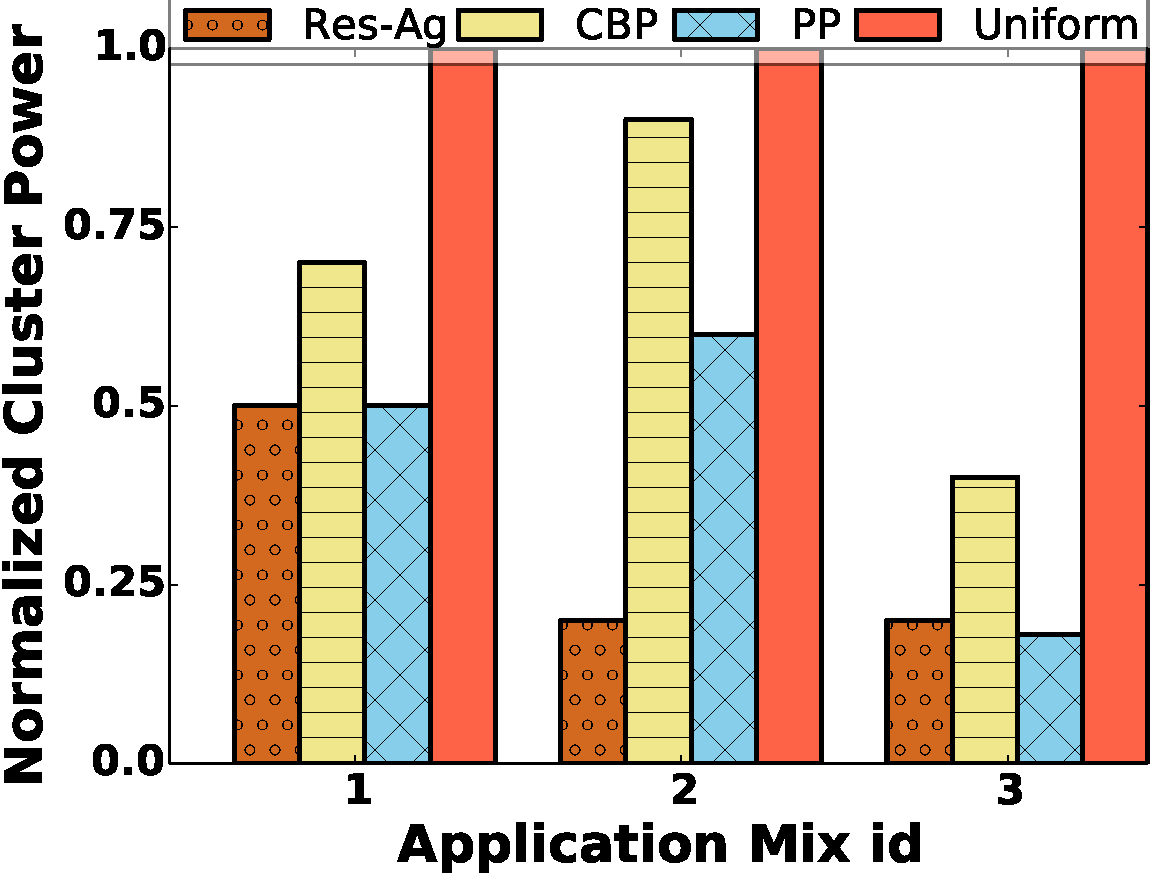
\includegraphics[width=.50\linewidth]{results/power.pdf}
%   \vspace{-2mm}
%   \caption{Normalized power.}
%   \label{fig:power}
% \end{wrapfigure}

% \begin{figure*}
%   \centering
%   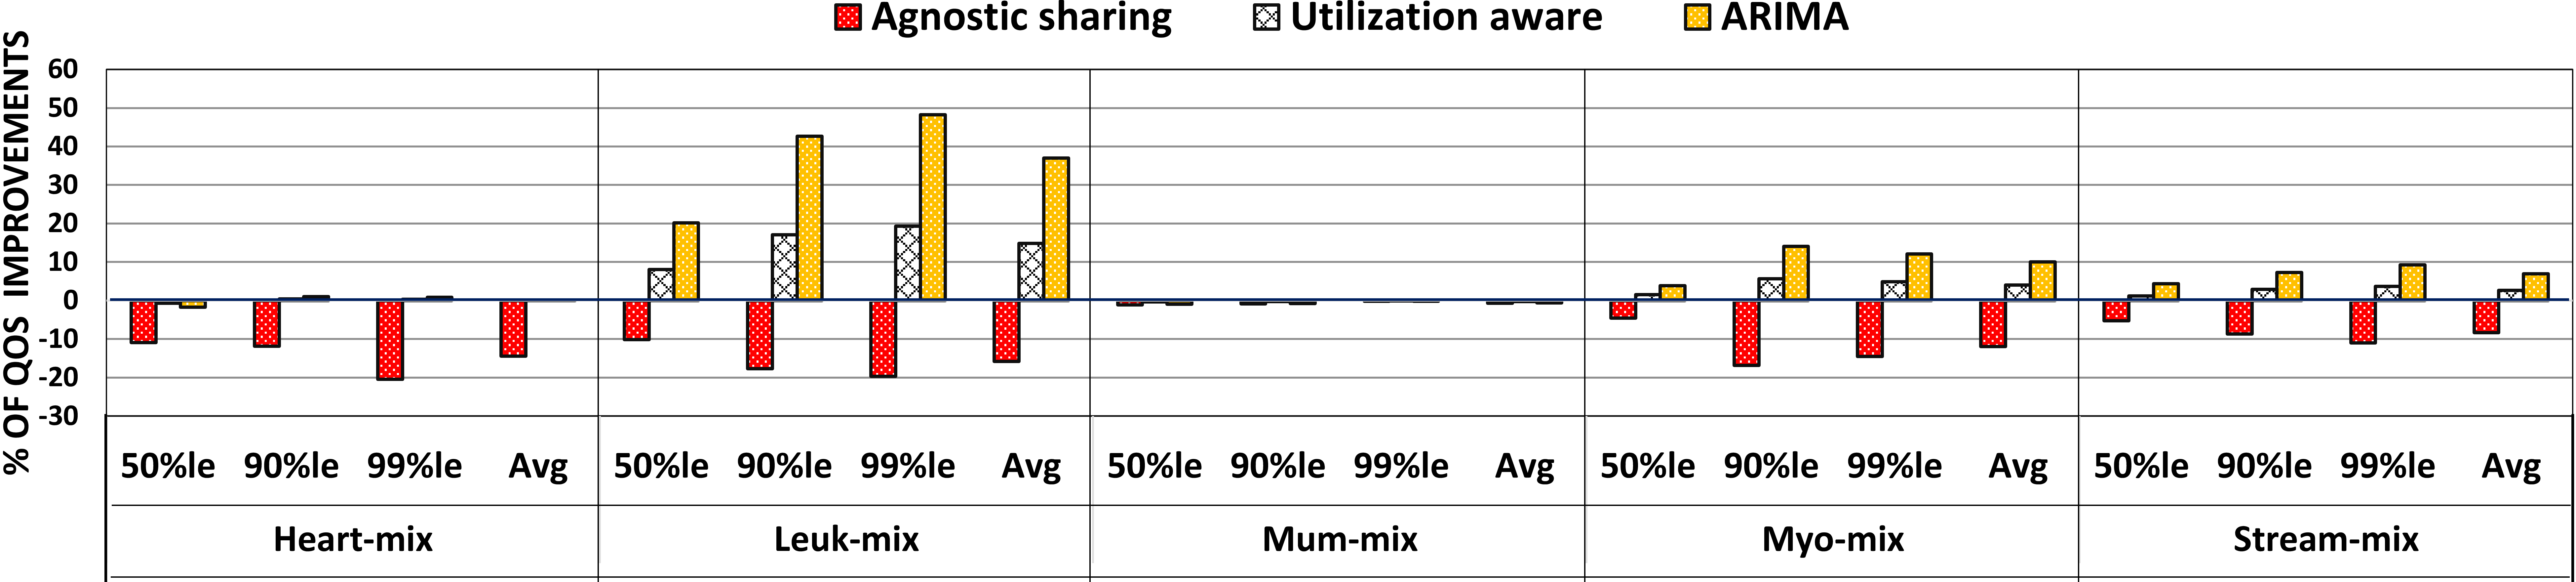
\includegraphics[width=.99\linewidth]{results/scheme.png}
%   \caption{50$^{th}$,90$^{th}$,99$^{th}$ and the average QoS variations plotted for different schedulers for representative mix of workloads compared against default FCFS scheduler.}
%   \label{fig:scheme}
% \end{figure*}

% \vspace{-0.2in}

~\subsection{Accuracy of the Peak Predictor}\label{sec:picking}
In case of PP scheduler, \textit{\textbf{d}} is the frequency at which the utilization aggregator at head-node is querying the worker nodes for GPU utilization that forms our time-series data. We vary the frequency at which we query the GPUs and plot the peak resource usage prediction accuracy in Figure~\ref{fig:accuracy}. As seen, PP improves its accuracy from 40\% to 84\% when the sampling interval for querying utilization is varied from 1000ms to 1 ms, beyond which the accuracy saturates. Hence for the maximum prediction accuracy, we set the utilization aggregator to query the GPU nodes every 1ms. The pyNVML overhead for querying the GPU at 1ms interval was minimal and does not affect the pod's performance. 

\begin{figure}[tbp!]
\begin{subfigure}[b]{.23\textwidth}
  \centering
   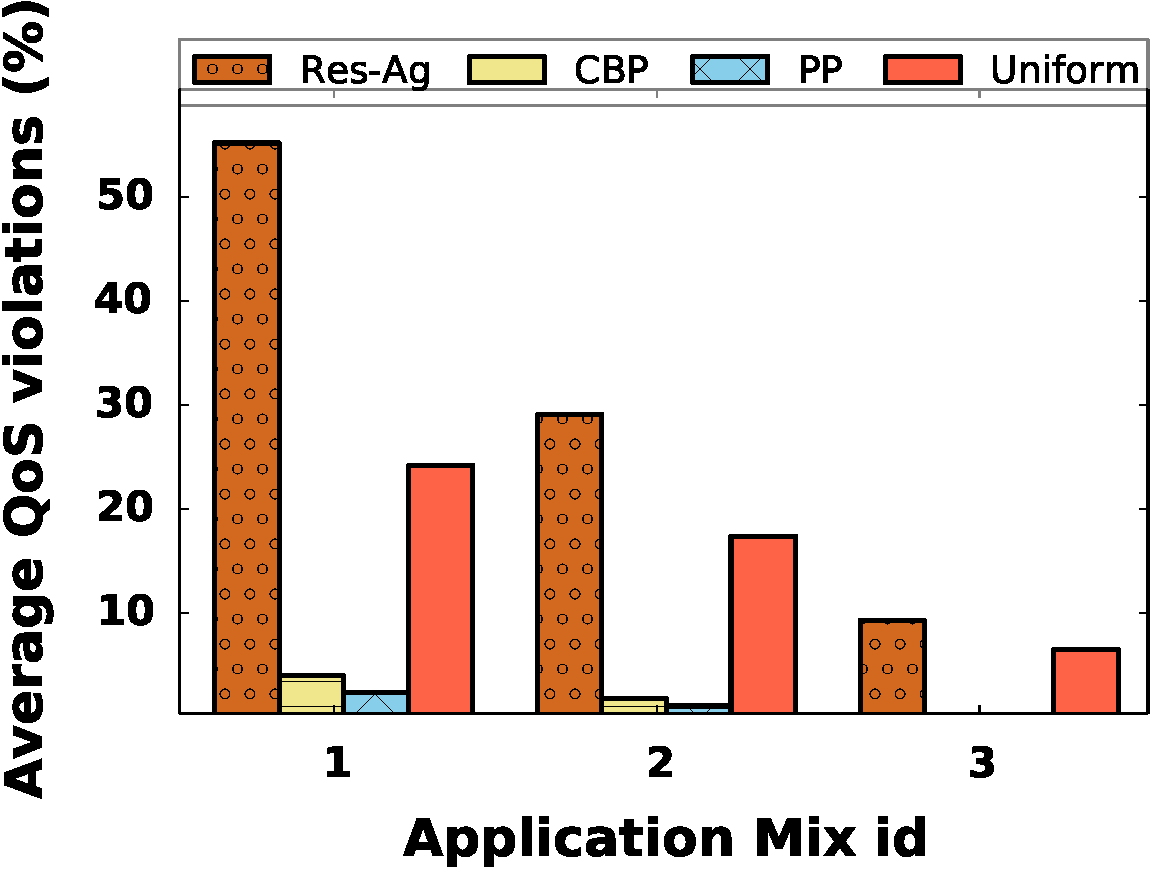
\includegraphics[width=.99\linewidth,height=3.3cm]{figs/qos-1.pdf}
  \caption{Average QoS violations per kilo inferences (queries).}
  \label{fig:qos}
\end{subfigure}
\begin{subfigure}[b]{.23\textwidth}
  \centering
  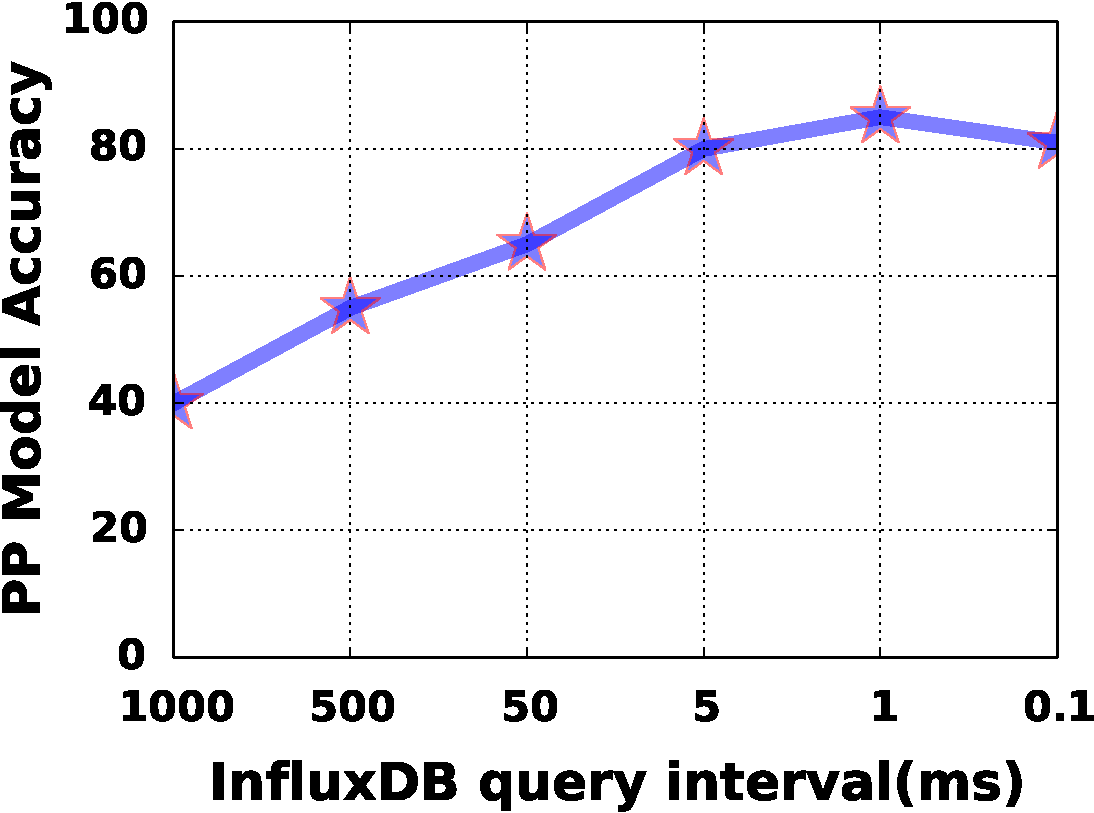
\includegraphics[width=.99\linewidth, height=3.3cm]{figs/accuracy.pdf}
  \caption{Accuracy of PP across varying time intervals in ms.}
  \label{fig:accuracy}
\end{subfigure}
\vspace{-3mm}
\caption{QoS guarantees and Accuracy of PP Scheduler.}
\label{fig:tuning}
\end{figure}

\begin{figure}[tbp!]
\begin{subfigure}[b]{.234\textwidth}
\centering
  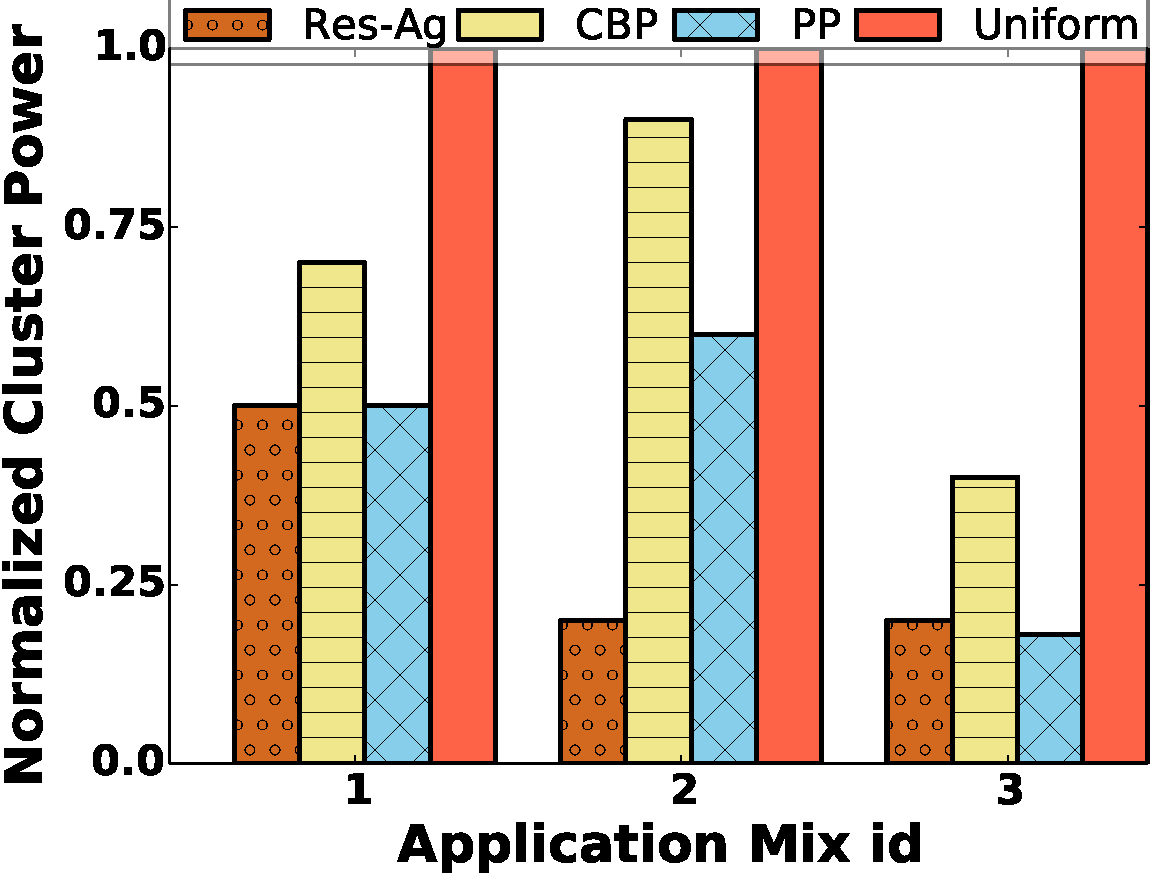
\includegraphics[width=.99\linewidth]{results/power.pdf}
  \caption{Normalized power comparisons across four schedulers.}
  \label{fig:power}
\end{subfigure}
\begin{subfigure}[b]{.234\textwidth}
\centering
  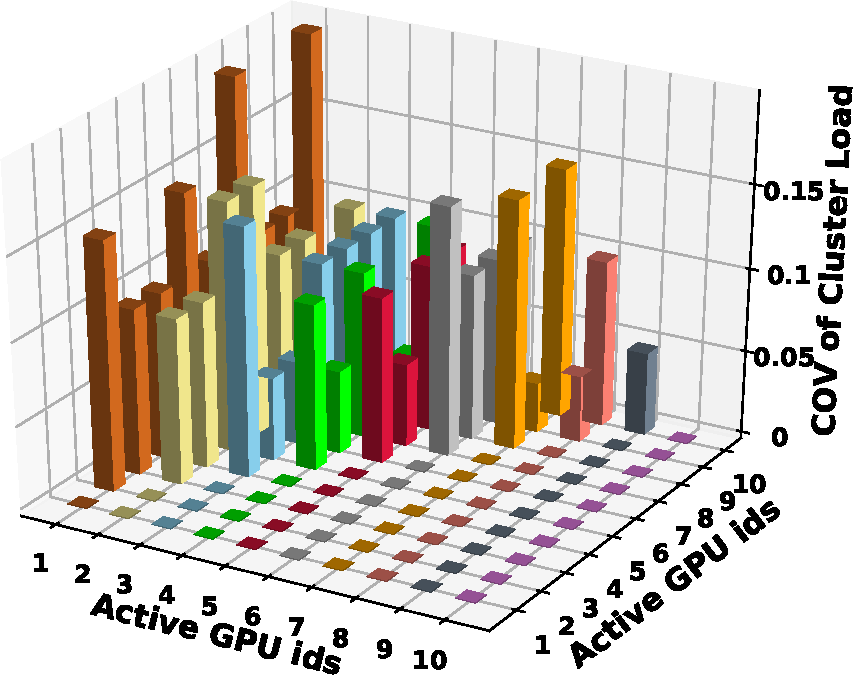
\includegraphics[width=.99\linewidth]{results/active3d.pdf}
  \caption{COV of SM-Load using CBP+PP for App-Mix-1.}
  \label{fig:load}
\end{subfigure}
\vspace{-2mm}
\caption{Cluster-wide Power savings and Load balancing.}
\label{fig:powandload}
\end{figure}



% \vspace{-0.15in}


\subsection{Discussion and Future Work}
\label{sec:overall}

An ideal scheduler would keep all 50/90/99$^{th}$ percentile and max utilization high for all the active GPUs. As a consequence, it yields the best performance per watt spent. This enables the scheduler to analyze different correlation metrics and consolidate the workloads/queries without violating the QoS. However, in reality, this scenario is impractical because of the varying inter-arrival times of GPU jobs submitted in a day. Therefore, the near-optimal solution would be, in every scheduling epoch the scheduler has to ensure performance aware bin-packing while, minimizing the GPU resource fragmentation. This leads to the energy efficient operating point which is achieved by the combination of CBP+PP scheduler.

Our proposed scheduling schemes can potentially be extended to any non-preemptible accelerators such as FPGAs, TPUs to improve the overall utilization while guaranteeing the QoS of the tasks. With the advent of distributed TF-based training~\cite{peng2018optimus,zhang2017slaq,qiao2017litz} on public-cloud GPUs, performance and utilization aware orchestration becomes inevitable to keep the costs low.  

% as input from device-level scheduling the approximate memory bandwidth of an application, by taking the ratio of the total data accesses by its computation kernels to the total time spent on the GPU. Workload balancing uses this information to avoid collocating bandwidth-bound threads. Resulting performance improvements leverage the fact that GPU-resident non-bandwidth/compute-bound threads can hide the memory latencies experienced by bandwidth-bound GPU kernels.


% eak uses a tail bound parameter PB to create the envelope whereas CBP uses a correlation cutoff parameter to identify if two applications are correlated. The baseline settings of all experimental parameters are listed in Table. 2. We evaluate the performance of the proposed methods in comparison with Existing methods based on dynamic consolidation. We run the Existing method with two different sizing functions: (i) Peak Existing sizes all applications based on their peak values and (ii) Mode Existing sizes all applications based on the mode of the distribution. There are three different objectives of consolidation: a)minimize power b) minimize the risk of consolidation (c) balance workload across active servers. We use the number of capacity violations as the metric for risk. To investigate load imbalance, we estimate the average CPU utilization for all active servers during the evaluation period and identify the server with the maximum average CPU utilization. The difference between the CPU utilization of the highest loaded server and the average utilization across all servers is taken as the metric for load imbalance.
% ~\subsubsection{Trading-off accuracy for performance}

%~\subsubsection{Load balancing \& Energy proportionality}
% Recall from the motivation energy plot. Workload Balancing: We next investigate the load balance across the active servers achieved by various methodologies. We observe that Mode Existing and CBP have servers that are always overloaded (average utilization of highest loaded server is 100\%) for AppSuite-1 and AppSuite-2. Such placement is not suitable in practice. Further, for all methodologies other than Peak , there is a large imbalance between the average utilization of the highest loaded server and the average utilization of the cluster. This is a direct consequence of the design of algorithms, where PP favors balancing, and the other algorithms favor creating a skew

%~\subsubsection{Algorithm scalability}

% We also simulate a placement where the initial number of virtual servers on a physical server is increased or decreased. Towards this purpose, we assume that the virtual servers are placed on a different capacity server of the same platform, i.e., with more or fewer processors as required for the simulation. Further, seasonal variations were observed in many workloads and hence, we increase and decrease the training period from the baseline setting. Finally, we vary the tuning parameters of CBP and PP and study their impact.

% ARIMA improves the QoS of service queries by up to 50\% compared to the baseline. This is due to the fact that it can forecast the GPU utilization metrics via the Knots interface. ARIMA does well in cases where the container usage load over time fits into a predictable growth function. This relationship between different load intervals positively correlating with each other could also be observed from the Spearman's correlation of Alibaba traces in Figure~\ref{fig:corr}, which also holds true for GPU.

% ~\subsection{Fragmentation}
% ~\subsubsection{Internal}
% Application managers like Tensorflow, Theano, Torch
% ~\subsubsection{External}
% Fragmentation: We next investigate the ability of CBP and PCP to deal with fragmentation ratio of application capacity to server capacity. We change the original servers in the data center and simulate placement on a larger number of lower capacity servers. In a heterogeneous setting where GPUs like K80 and M40 could be used to reduce external fragmentation issues.








